\documentclass[conference]{IEEEtran}
\IEEEoverridecommandlockouts
% The preceding line is only needed to identify funding in the first footnote. If that is unneeded, please comment it out.
\usepackage{cite}
\usepackage{amsmath,amssymb,amsfonts}
\usepackage{algorithm2e}
\usepackage{caption}
\usepackage{graphicx}
\usepackage{textcomp}
\usepackage{xcolor}
\def\BibTeX{{\rm B\kern-.05em{\sc i\kern-.025em b}\kern-.08em
    T\kern-.1667em\lower.7ex\hbox{E}\kern-.125emX}}
\graphicspath{ {images/} }
\begin{document}

\title{ENPM 661 Final Report\\}

\author{\IEEEauthorblockN{1\textsuperscript{st} Grayson Gilbert}
\IEEEauthorblockA{\textit{University of Maryland} \\
Annapolis, MD, United States \\
ggilbert@umd.edu}
\and
\IEEEauthorblockN{2\textsuperscript{nd} Marcus Hurt}
\IEEEauthorblockA{\textit{University of Maryland} \\
City, Country \\
email address or ORCID}
\and
\IEEEauthorblockN{3\textsuperscript{rd} Erebus Oh}
\IEEEauthorblockA{\textit{University of Maryland} \\
College Park, MD, United States \\
eoh12@umd.edu}
}

\maketitle

\begin{abstract}
This document is a model and instructions for \LaTeX.
This and the IEEEtran.cls file define the components of your paper [title, text, heads, etc.]. *CRITICAL: Do Not Use Symbols, Special Characters, Footnotes, 
or Math in Paper Title or Abstract.
\end{abstract}

\begin{IEEEkeywords}
component, formatting, style, styling, insert
\end{IEEEkeywords}

\section{Introduction}
Path planning is a fundamental challenge in robotics, particularly in highly complex environments or spaces with narrow passages. Sampling-based algorithms such as Rapidly-Exploring Random Trees (RRT) and other, faster variants like RRT-Connect, are widely used for their efficiency in exploring large configuration spaces \cite{b1, b2}. However, these methods often struggle in environments with narrow gaps between obstacles due to limited sampling in critical areas. Algorithms like Rapidly-Exploring Random Vines (RRV) can enhance performance in these scenarios using techniques like Principal Component Analysis (PCA) \cite{b3}. However, they tend to suffer from increased computation time and sensitivity to environmental structure. To address these limitations, the adaptive RRT-Connect (ARRT-Connect) algorithm was developed, which combines greedy sampling, local environment analysis, and a flexible bidirectional expansion strategy \cite{b4}. For this project, ARRT-Connect was re-implemented and tested on the competition map developed in Project 3. After refining the algorithm in a 2D environment, ARRT-Connect was further tested in a Gazebo simulation using TurtleBot3. The results demonstrate that ARRT-Connect significantly improves planning efficiency and robustness in both simulated and practical settings, particularly in environments that include narrow passages and cluttered regions.

\section{Background}
Rapidly Random Tree* (RRT*) has been proven effective for domains with non-holonomic constraints and/or high dimensionality \cite{b5}. The process involves pathing towards randomly sampled points in the workspace. This is especially useful in unknown or very large environments where performing a classic search algorithm (Dijkstra, A*, etc) would be too slow or inefficient.

However, due to RRT*'s randomness in sampling points in the workspace, it is susceptible to unlucky sampling leading to inefficient search. Thus, many improvements on RRT have been proposed over the years since 1998 for a more robust sampling searching algorithm.

RRT-Connect is an improvement on RRT, since it performs bidirectional search from the start and goal nodes\cite{b2}. A further improvement on RRT-Connect is Adaptive RRT-Connect, which is what we will be implementing in Project 5. ARRT-Connect introduces a greedier sampler and a more efficient tree expanding algorithm to better judge potentially promising nodes\cite{b4}.

\subsection{ARRT-Connect Algorithm}

% %% Algorithm 1: ARRT-Connect

\begin{figure}[!t]
  \centering
  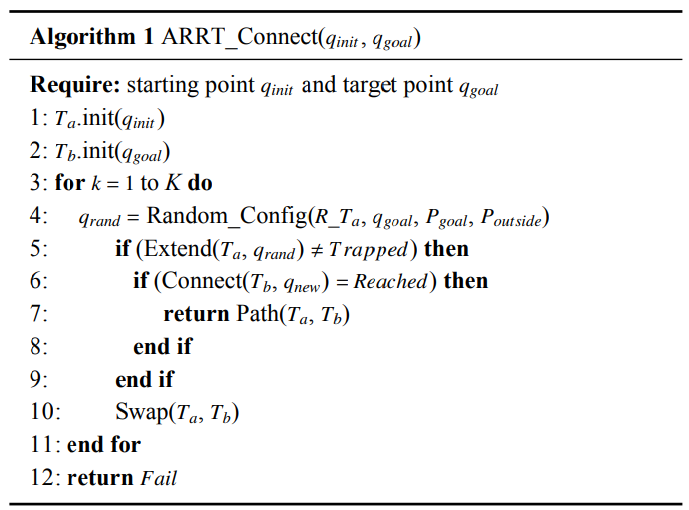
\includegraphics[width=\linewidth]{algorithm1}  % Replace with your image filename
  \caption{RRT-Connect/ARRT-Connect Method}
  \label{fig:five}
\end{figure}


% %% Algorithm 2: Connect

\begin{figure}[!t]
  \centering
  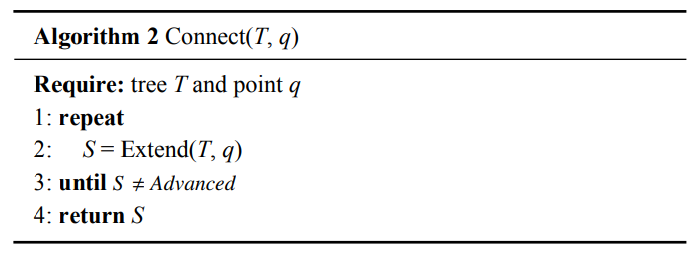
\includegraphics[width=\linewidth]{algorithm2}  % Replace with your image filename
  \caption{Connect Method}
  \label{fig:three}
\end{figure}

ARRT-Connect is identical to RRT-Connect as shown in Algorithm 1 and 2 in Figures \ref{fig:three} and \ref{fig:five}, respectively. The novel changes are shown in Random\_Config, Extend, and Swap.


% %% Algorithm 3: Random_Config


\begin{figure}[!t]
  \centering
  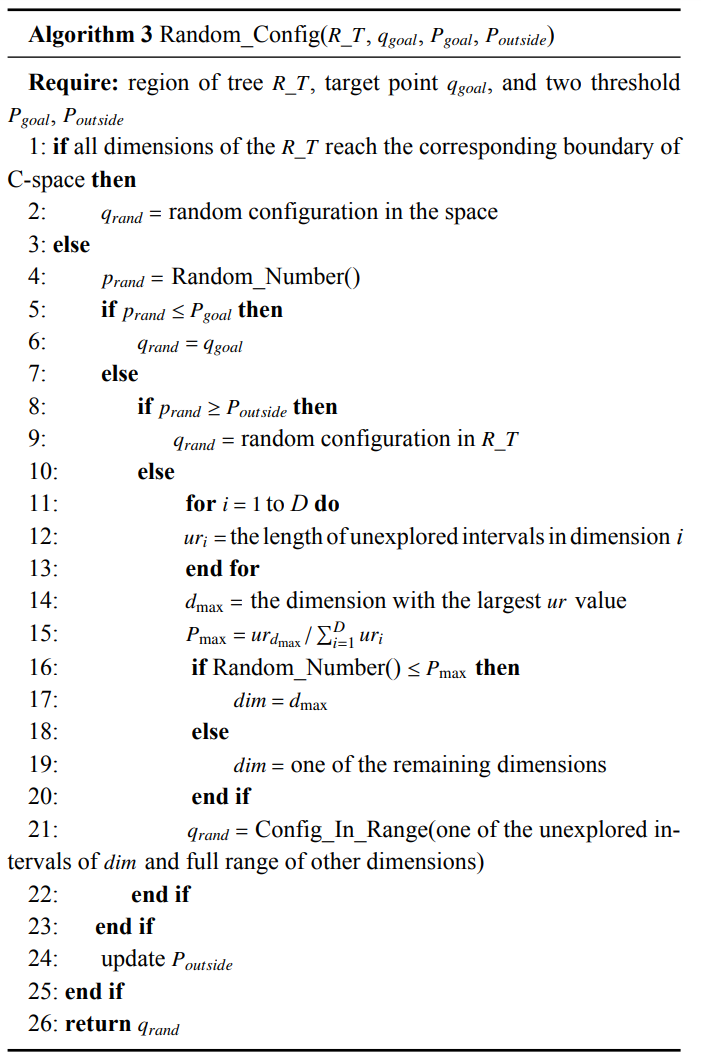
\includegraphics[width=\linewidth]{algorithm3}  % Replace with your image filename
  \caption{\text{Random\_Config Method}}
  \label{fig:four}
\end{figure}

Instead of a randomly uniform sampler, as seen in RRT-Connect, we use a greedy sampler in Figure \ref{fig:four}, Algorithm 3. This sampler updates the sampling area to increase the probability that a new sample will be an unexplored area (that will change the sampling area) rather than remain in the current sampling area. This greedy sampler aims to both accelerate tree expansion and workspace resolution to find an optimal path.

%% Algorithm 4: Extend

\begin{figure}[!t]
  \centering
  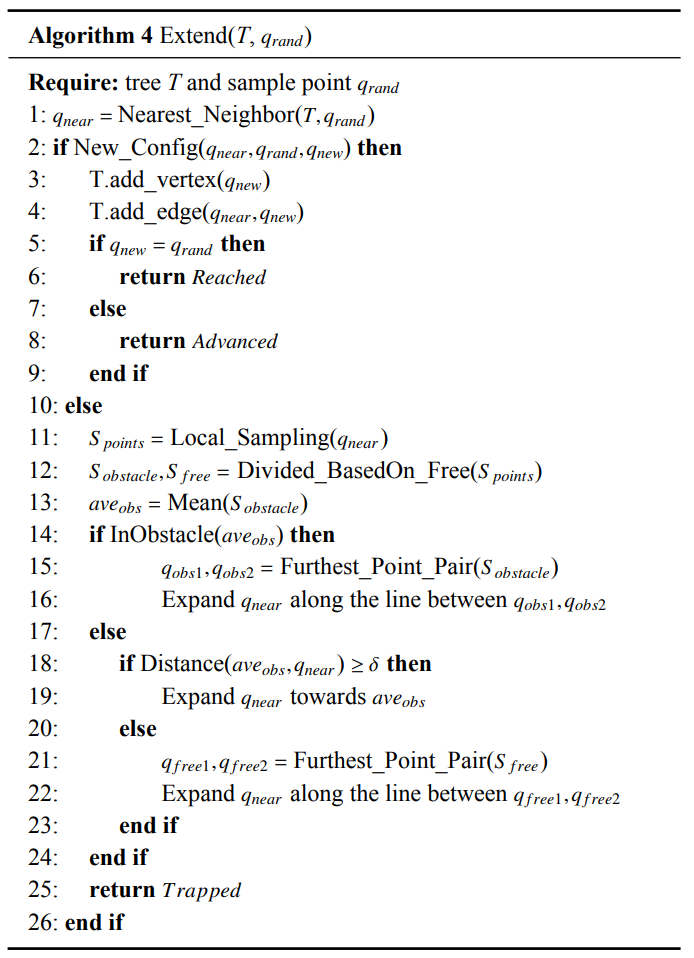
\includegraphics[width=\linewidth]{algorithm4}  % Replace with your image filename
  \caption{Extend Method}
  \label{fig:two}
\end{figure}

\begin{figure}[!t]
  \centering
  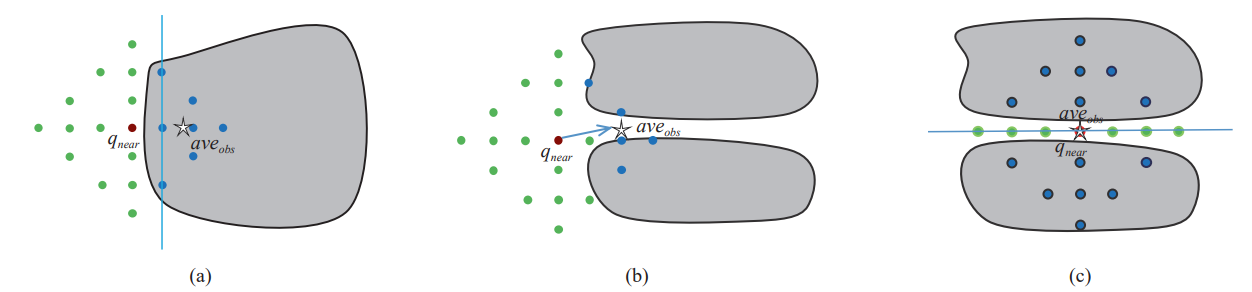
\includegraphics[width=\linewidth]{extend-scenarios}  % Replace with your image filename
  \caption{Extend Scenarios}
  \label{fig:extend-scenarios}
\end{figure}

After getting a random sample from Random\_Config, we attempt the normal RRT-Connect connection method of connecting the sample to closest node on the tree. However, if that is not possible (an obstacle is blocking the way), then the Extend method will calculate which of three scenarios it is in. This calculation is done by local sampling around the closest node to the random sample, and dividing local samples into two groups: in free space or in obstacle space. The average location for the group of obstacle samples is calculated and informs us of what scenario we are in. The three scenarios are depicted in Figure \ref{fig:extend-scenarios}.

If the average obstacle point is in the obstacle space, then it is a Wall scenario. Then, the furthest two points in the obstacle group of local samples creates a line that we search to find the next free space sample.

If the average obstacle point is in free space, we then check the distance between the closest node and the average obstacle point. If this distance is relatively big, then we are at an entrance to a narrow passage, which means the tree should try to expand towards the average obstacle point. If the distance between the closest node and average obstacle point is small, then we are in a narrow passage. The two farthest points in the free space local sampling group indicates our direction of expansion. 

\ref{fig:two}

%% Algorithm 5: Swap

\begin{figure}[!t]
  \centering
  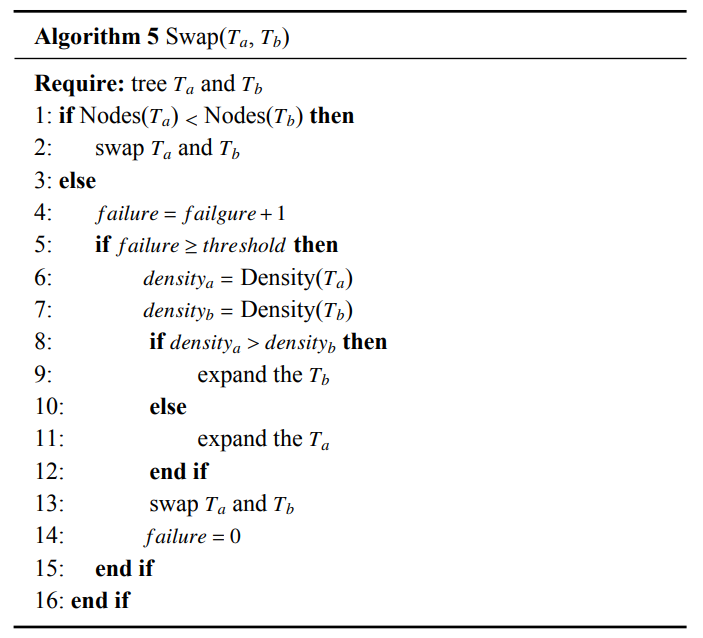
\includegraphics[width=\linewidth]{algorithm5}  % Replace with your image filename
  \caption{Swap Method}
  \label{fig:one}
\end{figure}

As shown in Figure \ref{fig:one}, Algorithm 5 is the last step in each iteration of ARRT-Connect. The Swap method determines which tree in the bidirectional search (either the one from the start or from the goal node) should be expanded next. It will try to choose the tree with the least nodes, but when that fails $threshold$ number of times, the method will choose the tree with the lowest density. 


\section{Methodology}

\section{Tests/demos/experimentation}

\section{Discussion}

\section{Conclusion}

We were able to successfully implement the ARRT-Connect algorithm in Python and ROS simulation, as well as prove its robustness in multiple scenarios involving environments with typically difficult obstacles for RRT-like algorithms such as walls and narrow passages.


\clearpage
\begin{thebibliography}{00}
% RRT
\bibitem{b1} S. M. Lavalle, “Rapidly-exploring random trees : A new tool for path planning,” Iowa State University, Tech. Repnewline. 98-11,Oct. 1998.
% RRT-Connect
\bibitem{b2} J. J. Kuffner and S. M. LaValle, “Rrt-connect: An efficient approach to single-query path planning,” in Proc. ICRA Millennium Conf. IEEE Int. Conf. Robotics and Automation, 2000, vol. 2, pp. 995–1001. 
% RRV
\bibitem{b3} A. Tahirovic and M. Ferizbegovic, “Rapidly-Exploring Random Vines (RRV) for motion planning in configuration spaces with narrow passages,” in Proc. IEEE Int. Conf. Robotics and Automation (ICRA), 2018, pp. 7055–7062, doi: 10.1109/ICRA.2018.8460186.
% ARRT-Connect
\bibitem{b4} B. Li and B. Chen, "An Adaptive Rapidly-Exploring Random Tree," in IEEE/CAA Journal of Automatica Sinica, vol. 9, no. 2, pp. 283-294, February 2022, doi: 10.1109/JAS.2021.1004252. 
% RRT*
\bibitem{b5} S. Karaman and E. Frazzoli, “Sampling-based algorithms for optimal motion planning,” Int. J. Robot. Res., vol. 30, no. 7, pp. 846–894, 2011.
\end{thebibliography}
\end{document}
